\PassOptionsToPackage{unicode}{hyperref}
\documentclass[aspectratio=1610, 11pt]{beamer}

\usepackage{amsmath}
\usepackage{amssymb}
\usetheme{tudo}

\title{Datenstrukturen, Algorithmen und Programmierung~2}
\author[A.~Coja-Oghlan]{Amin Coja-Oghlan}
\institute[DAP2]{Lehrstuhl Informatik 2\\Fakult\"at f\"ur Informatik}

\newcommand\dist{\mathrm{dist}}
\renewcommand{\vec}[1]{\boldsymbol{#1}}
\newcommand\NULL{{\tt NULL}}
\newcommand\dd{\mathrm d}
\newcommand\eul{\mathrm e}
\newcommand\cA{\mathcal A}
\newcommand\cB{\mathcal B}
\newcommand\cC{\mathcal C}
\newcommand\cD{\mathcal D}
\newcommand\cE{\mathcal E}
\newcommand\cF{\mathcal F}
\newcommand\cG{\mathcal G}
\newcommand\cH{\mathcal H}
\newcommand\cI{\mathcal I}
\newcommand\cJ{\mathcal J}
\newcommand\cK{\mathcal K}
\newcommand\cL{\mathcal L}
\newcommand\cM{\mathcal M}
\newcommand\cN{\mathcal N}
\newcommand\cO{\mathcal O}
\newcommand\cP{\mathcal P}
\newcommand\cQ{\mathcal Q}
\newcommand\cR{\mathcal R}
\newcommand\cS{\mathcal S}
\newcommand\cT{\mathcal T}
\newcommand\cU{\mathcal U}
\newcommand\cV{\mathcal V}
\newcommand\cW{\mathcal W}
\newcommand\cX{\mathcal X}
\newcommand\cY{\mathcal Y}
\newcommand\cZ{\mathcal Z}
\newcommand\fA{\mathfrak A}
\newcommand\fB{\mathfrak B}
\newcommand\fC{\mathfrak C}
\newcommand\fD{\mathfrak D}
\newcommand\fE{\mathfrak E}
\newcommand\fF{\mathfrak F}
\newcommand\fG{\mathfrak G}
\newcommand\fH{\mathfrak H}
\newcommand\fI{\mathfrak I}
\newcommand\fJ{\mathfrak J}
\newcommand\fK{\mathfrak K}
\newcommand\fL{\mathfrak L}
\newcommand\fM{\mathfrak M}
\newcommand\fN{\mathfrak N}
\newcommand\fO{\mathfrak O}
\newcommand\fP{\mathfrak P}
\newcommand\fQ{\mathfrak Q}
\newcommand\fR{\mathfrak R}
\newcommand\fS{\mathfrak S}
\newcommand\fT{\mathfrak T}
\newcommand\fU{\mathfrak U}
\newcommand\fV{\mathfrak V}
\newcommand\fW{\mathfrak W}
\newcommand\fX{\mathfrak X}
\newcommand\fY{\mathfrak Y}
\newcommand\fZ{\mathfrak Z}
\newcommand\fa{\mathfrak a}
\newcommand\fb{\mathfrak b}
\newcommand\fc{\mathfrak c}
\newcommand\fd{\mathfrak d}
\newcommand\fe{\mathfrak e}
\newcommand\ff{\mathfrak f}
\newcommand\fg{\mathfrak g}
\newcommand\fh{\mathfrak h}
%\newcommand\fi{\mathfrak i}
\newcommand\fj{\mathfrak j}
\newcommand\fk{\mathfrak k}
\newcommand\fl{\mathfrak l}
\newcommand\fm{\mathfrak m}
\newcommand\fn{\mathfrak n}
\newcommand\fo{\mathfrak o}
\newcommand\fp{\mathfrak p}
\newcommand\fq{\mathfrak q}
\newcommand\fr{\mathfrak r}
\newcommand\fs{\mathfrak s}
\newcommand\ft{\mathfrak t}
\newcommand\fu{\mathfrak u}
\newcommand\fv{\mathfrak v}
\newcommand\fw{\mathfrak w}
\newcommand\fx{\mathfrak x}
\newcommand\fy{\mathfrak y}
\newcommand\fz{\mathfrak z}
\newcommand\vA{\vec A}
\newcommand\vB{\vec B}
\newcommand\vC{\vec C}
\newcommand\vD{\vec D}
\newcommand\vE{\vec E}
\newcommand\vF{\vec F}
\newcommand\vG{\vec G}
\newcommand\vH{\vec H}
\newcommand\vI{\vec I}
\newcommand\vJ{\vec J}
\newcommand\vK{\vec K}
\newcommand\vL{\vec L}
\newcommand\vM{\vec M}
\newcommand\vN{\vec N}
\newcommand\vO{\vec O}
\newcommand\vP{\vec P}
\newcommand\vQ{\vec Q}
\newcommand\vR{\vec R}
\newcommand\vS{\vec S}
\newcommand\vT{\vec T}
\newcommand\vU{\vec U}
\newcommand\vV{\vec V}
\newcommand\vW{\vec W}
\newcommand\vX{\vec X}
\newcommand\vY{\vec Y}
\newcommand\vZ{\vec Z}
\newcommand\va{\vec a}
\newcommand\vb{\vec b}
\newcommand\vc{\vec c}
\newcommand\vd{\vec d}
\newcommand\ve{\vec e}
\newcommand\vf{\vec f}
\newcommand\vg{\vec g}
\newcommand\vh{\vec h}
\newcommand\vi{\vec i}
\newcommand\vj{\vec j}
\newcommand\vk{\vec k}
\newcommand\vl{\vec l}
\newcommand\vm{\vec m}
\newcommand\vn{\vec n}
\newcommand\vo{\vec o}
\newcommand\vp{\vec p}
\newcommand\vq{\vec q}
\newcommand\vr{\vec r}
\newcommand\vs{\vec s}
\newcommand\vt{\vec t}
\newcommand\vu{\vec u}
\renewcommand\vv{\vec v}
\newcommand\vw{\vec w}
\newcommand\vx{\vec x}
\newcommand\vy{\vec y}
\newcommand\vz{\vec z}
\renewcommand\AA{\mathbb A}
\newcommand\NN{\mathbb N}
\newcommand\ZZ{\mathbb Z}
\newcommand\PP{\mathbb P}
\newcommand\QQ{\mathbb Q}
\newcommand\RR{\mathbb R}
\newcommand\RRpos{\mathbb R_{\geq0}}
\newcommand\QQpos{\mathbb Q_{\geq0}}
\renewcommand\SS{\mathbb S}
\newcommand\CC{\mathbb C}
\newcommand{\ord}{\mathrm{ord}}
\newcommand{\id}{\mathrm{id}}
\newcommand{\pr}{\mathrm{P}}
\newcommand{\Vol}{\mathrm{vol}}
\newcommand\norm[1]{\left\|{#1}\right\|} 
\newcommand\sign{\mathrm{sign}}
\newcommand{\eps}{\varepsilon}
\newcommand{\abs}[1]{\left|#1\right|}
\newcommand\bc[1]{\left({#1}\right)} 
\newcommand\cbc[1]{\left\{{#1}\right\}} 
\newcommand\bcfr[2]{\bc{\frac{#1}{#2}}} 
\newcommand{\bck}[1]{\left\langle{#1}\right\rangle} 
\newcommand\brk[1]{\left\lbrack{#1}\right\rbrack} 
\newcommand\scal[2]{\bck{{#1},{#2}}} 
\newcommand{\vecone}{\mathbb{1}}
\newcommand{\tensor}{\otimes}
\newcommand{\diag}{\mathrm{diag}}
\newcommand{\ggt}{\mathrm{ggT}}
\newcommand{\kgv}{\mathrm{kgV}}
\newcommand{\trans}{\top}
\newcommand{\Karonski}{Karo\'nski}
\newcommand{\Erdos}{Erd\H{o}s}
\newcommand{\Renyi}{R\'enyi}
\newcommand{\Lovasz}{Lov\'asz}
\newcommand{\Juhasz}{Juh\'asz}
\newcommand{\Bollobas}{Bollob\'as}
\newcommand{\Furedi}{F\"uredi}
\newcommand{\Komlos}{Koml\'os}
\newcommand{\Luczak}{\L uczak}
\newcommand{\Kucera}{Ku\v{c}era}
\newcommand{\Szemeredi}{Szemer\'edi}

\newcommand{\mytitle}{Netzwerkfl\"usse}

\begin{document}

\frame[plain]{\titlepage}

\begin{frame}\frametitle{\mytitle}
	\begin{exampleblock}{Worum geht es?}
		\begin{itemize}
			\item ein Netzwerk ist ein gerichteter Graph mit Kantenkapazit\"aten
			\item welche maximale Ladung kann von einer Quelle zu einer Senke transportiert werden?
			\item \emph{Anwendung:} Matchings in bipartiten Graphen
		\end{itemize}
	\end{exampleblock}
\end{frame}

\begin{frame}\frametitle{\mytitle}
	\begin{overprint}
		\onslide<1>
		\begin{block}{Definition}
			Ein (endlicher) \alert{gerichteter Graph} $G$ besteht aus
			\begin{itemize}
				\item einer endlichen Menge $V(G)$ von \alert{Knoten} und
				\item einer Menge $E(G)\subseteq V(G)\times V(G)$ von \alert{gerichteten Kanten}
			\end{itemize}
			Eine Kante der Form $(v,v)$ nennt man \alert{Schleife}
		\end{block}
		\onslide<2>
		\begin{exampleblock}{Notation}
			\begin{itemize}
				\item wir bezeichnen mit
					\begin{align*}
						\partial^+v&=\partial_G^+v=\{w\in V:(w,v)\in E(G)\},&\partial^-v&=\partial_G^-v=\{w\in V:(v,w)\in E(G)\}
					\end{align*}
					die eingehende und die ausgehende Nachbarschaft von $v$
				\item ferner definiere
					\begin{align*}
						d^+_G(v)&=|\partial^+_Gv|,&d^-_G(v)&=|\partial^-_Gv|
					\end{align*}
					als den eingehenden und den ausgehenden Grad von $v$
			\end{itemize}
		\end{exampleblock}
		\onslide<3>
		\begin{exampleblock}{Breitensuche}
			\begin{itemize}
				\item wir haben {\tt BFS} f\"ur ungerichtete Graphen kennengelernt
				\item der Algorithmus \"ubertr\"agt sich auf gerichtete Graphen, indem in der Hauptschleife (Schritt 8) nur $u\in\partial^-v$ in die Warteschlange eingef\"ugt werden
				\item der Algorithmus bestimmt dann k\"urzeste \emph{gerichtete} Pfade in $G$
			\end{itemize}
		\end{exampleblock}
	\end{overprint}
\end{frame}

\begin{frame}\frametitle{\mytitle}
	\begin{overprint}
		\onslide<1>
		\begin{block}{Definition}
			Ein \alert{Netzwerk} $N=(G,c,s,t)$ besteht aus
			\begin{itemize}
				\item einem gerichteten Graphen $G$
				\item einer Kapazit\"atsfunktion $c:V\times V\to\RRpos$, so da\ss
					$$c(v,w)=0\quad\mbox{falls }(v,w)\not\in E(G)$$
				\item einer Quelle $s\in V(G)$
				\item einer Senke $t\in V(G)\setminus\{s\}$
			\end{itemize}
		\end{block}
		\onslide<2>
		\begin{exampleblock}{Definition}
			Ein \alert{Flu\ss} in einem Netzwerk $N$ ist eine Funktion $f:V\times V\to\RR$, so da\ss
			\begin{itemize}
				\item $f(v,w)\leq c(v,w)$ f\"ur alle $v,w\in V(G)$
				\item $f(v,w)+f(w,v)=0$ f\"ur alle $v,w\in V(G)$
				\item $\sum_{w\in V(G)}f(v,w)=0$ f\"ur alle $v\in V(G)\setminus\{s,t\}$
			\end{itemize}
			Der \alert{Wert} von $f$ ist definiert als
			\begin{align*}
				|f|&=\sum_{w\in V(G)}f(s,w)
			\end{align*}
		\end{exampleblock}
		\onslide<3>
		\begin{exampleblock}{Notation}
			F\"ur eine Funktion $f:V\times V\to \RR$, $v\in V$ und $A,B\subset V$ definieren wir
			\begin{align*}
				f(v,A)&=\sum_{w\in A}f(v,w)\\
				f(A,v)&=\sum_{w\in A}f(w,v)\\
				f(A,B)&=\sum_{v\in A}\sum_{w\in B}f(v,w)
			\end{align*}
		\end{exampleblock}
		\onslide<5>
		\begin{exampleblock}{Das Max Flow-Problem}
			\begin{itemize}
				\item gegeben ist ein Netzwerk $N$
				\item das Ziel ist, einen Flu\ss\ mit maximalem Wert (einen ``maximalen Flu\ss'') zu bestimmen
				\item die Idee ist, ausgehend vom Nullflu\ss\ den aktuellen Flu\ss\ immer weiter zu ``augmentieren''
			\end{itemize}
		\end{exampleblock}
		\onslide<4>
		\begin{block}{Lemma}
			Sei $N$ ein Netzwerk und $f$ ein Flu\ss.
			F\"ur alle $A,B,W\subseteq V$ gilt
			\begin{align*}
				f(A,A)&=0\\
				f(A,B)+f(B,A)&=0\\
				f(A\cup B,C)&=f(A,C)+f(B,C)&&\mbox{sofern }A\cap B=\emptyset\\
				f(C,A\cup B)&=f(C,A)+f(C,B)&&\mbox{sofern }A\cap B=\emptyset
			\end{align*}
		\end{block}
	\end{overprint}
\end{frame}

\begin{frame}\frametitle{\mytitle}
	\begin{overprint}
		\onslide<1>
		\begin{exampleblock}{Restfl\"usse}
			Sei $N$ ein Netzwerk und $f$ ein Flu\ss
			\begin{itemize}
				\item die \alert{Restkapazit\"at} von $f$ in $N$ ist definiert als
					$$c_f(v,w)=c(v,w)-f(v,w)\qquad(v,w\in V(G))$$
				\item das \alert{Restnetzwerk} von $f$ in $N$ ist das Netzwerk mit Kantenkapazit\"atsfunktion $c_f$ und Kantenmenge
					$$E_f=\cbc{(v,w)\in V(G):c_f(v,w)>0}$$
			\end{itemize}
		\end{exampleblock}
		\onslide<2>
		\begin{block}{Lemma}
			Angenommen $N$ ist ein Netzwerk, $f$ ist ein Flu\ss\ in $N$ und $g$ ist ein Flu\ss\ in $N_f$.
			Dann ist $f+g$ ein Flu\ss\ in $N$ mit Wert $|f+g|=|f|+|g|$.
		\end{block}
	\end{overprint}
\end{frame}

\begin{frame}\frametitle{\mytitle}
	\begin{overprint}
		\onslide<1>
		\begin{exampleblock}{Augmentierende Pfade}
			\begin{itemize}
				\item ein \alert{$f$-augmentierender Pfad} in $N$ ist ein $s$-$t$-Pfad in $N_f$
				\item die \alert{Kapazit\"at} eines solchen Pfades $p$ ist
					\begin{align*}
						c_f(p)&=\min\{c_f(u,v):(u,v)\mbox{ ist eine Kante auf }p\}>0
					\end{align*}
			\end{itemize}
		\end{exampleblock}
		\onslide<2>
		\begin{center} 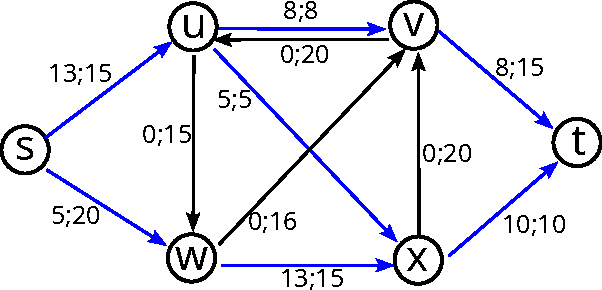
\includegraphics[height=40mm]{./images/flow1.pdf} \end{center}
		\begin{exampleblock}{Beispiel}
			\begin{itemize}
				\item ein Netzwerkflu\ss\ $f$
			\end{itemize}
		\end{exampleblock}
		\onslide<3>
		\begin{center} 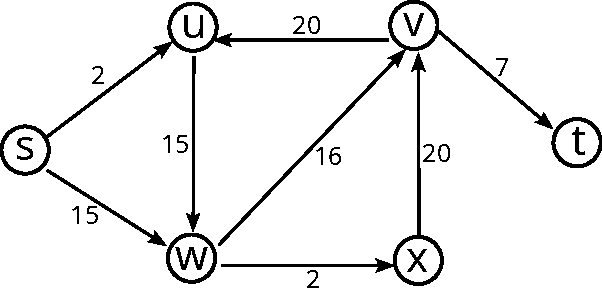
\includegraphics[height=40mm]{./images/flow2.pdf} \end{center}
		\begin{exampleblock}{Beispiel}
			\begin{itemize}
				\item das Restnetzwerk $N_f$
			\end{itemize}
		\end{exampleblock}
		\onslide<4>
		\begin{center} 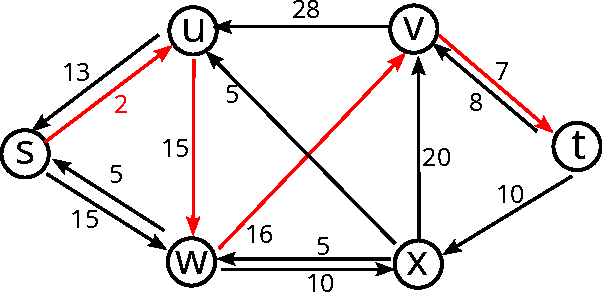
\includegraphics[height=40mm]{./images/flow3.pdf} \end{center}
		\begin{exampleblock}{Beispiel}
			\begin{itemize}
				\item ein augmentierender Pfad der Kapazit\"at zwei
			\end{itemize}
		\end{exampleblock}
		\onslide<5>
		\begin{block}{Lemma}
			Angenommen $N$ ist ein Netzwerk, $f$ ein Flu\ss\ und $p$ ein augmentierender Pfad.
			Dann ist $f_p:V\times V\to\RR$ mit
			\begin{align*}
				f_p(v,w)=\bc{\vecone\{(v,w)\mbox{ ist Kante von }p\}-\vecone\{(w,v)\mbox{ ist Kante von }p\}}c_f(p)
			\end{align*}
			ein Flu\ss\ mit Wert $c_f(p)$ in $N_f$
		\end{block}
		\onslide<6>
		\begin{block}{Korollar}
			Angenommen $N$ ist ein Netzwerk, $f$ ein Flu\ss\ und $p$ ein augmentierender Pfad.
			Dann ist $f+f_p$ ein Flu\ss\ in $N$ mit Wert $|f|+c_f(p)>|f|$.
		\end{block}
	\end{overprint}
\end{frame}

\begin{frame}\frametitle{\mytitle}
	\begin{overprint}
		\onslide<1>
		\begin{exampleblock}{Algorithmus {\tt FordFulkerson}}
			\begin{enumerate}
				\item setze $f(v,w)=0$ f\"ur alle $v,w\in V$
				\item solange es einen augmentierenden Pfad $p$ in $N_f$ gibt
				\item $\qquad$setze $f=f+f_p$
				\item gib $f$ aus
			\end{enumerate}
		\end{exampleblock}
		\onslide<2>
		\begin{exampleblock}{Anmerkungen}
			\begin{itemize}
				\item der Algorithmus spezifiziert nicht, wie/welcher Pfad $p$ gefunden wird
				\item es ist nicht klar, da\ss\ der Algorithmus h\"alt!
				\item sofern alle Kapazit\"aten ganz sind, ist das aber der Fall
			\end{itemize}
		\end{exampleblock}
		\onslide<3>
		\begin{center}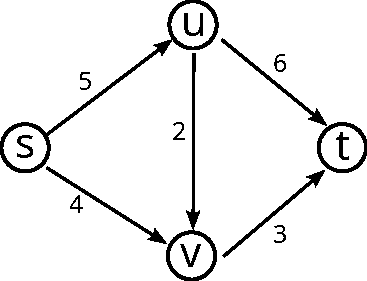
\includegraphics[height=40mm]{./images/flow4.pdf}\end{center}
\begin{exampleblock}{Beispiel}
			\begin{itemize}
				\item das urspr\"ungliche Netzwerk
			\end{itemize}
		\end{exampleblock}
		\onslide<4>
		\begin{center}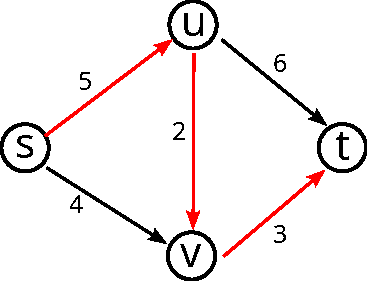
\includegraphics[height=40mm]{./images/flow5.pdf}\end{center}
\begin{exampleblock}{Beispiel}
			\begin{itemize}
				\item ein augmentierender Pfad der Kapazit\"at zwei
			\end{itemize}
		\end{exampleblock}
		\onslide<5>
		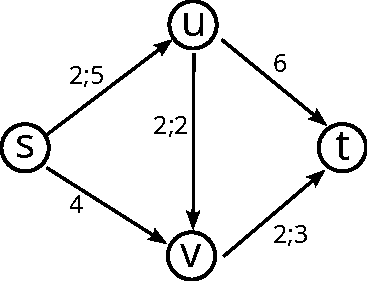
\includegraphics[height=40mm]{./images/flow7.pdf}\hfill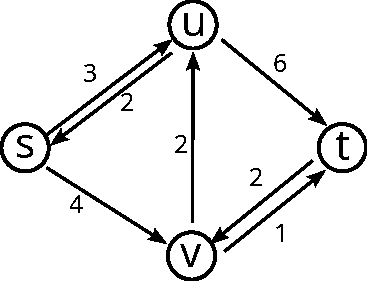
\includegraphics[height=40mm]{./images/flow6.pdf}
\begin{exampleblock}{Beispiel}
			\begin{itemize}
				\item links: der aktuelle Flu\ss\ im Ursprungsnetzwerk
				\item rechts: das Restnetzwerk
			\end{itemize}
		\end{exampleblock}
		\onslide<6>
		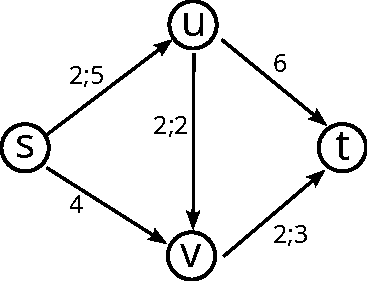
\includegraphics[height=40mm]{./images/flow7.pdf}\hfill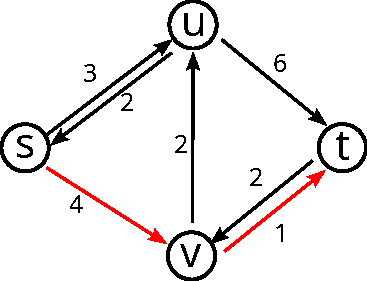
\includegraphics[height=40mm]{./images/flow8.pdf}
\begin{exampleblock}{Beispiel}
			\begin{itemize}
				\item links: der aktuelle Flu\ss\ im Ursprungsnetzwerk
				\item rechts: ein augmentierender Pfad mit Kapazit\"at eins
			\end{itemize}
		\end{exampleblock}
		\onslide<7>
		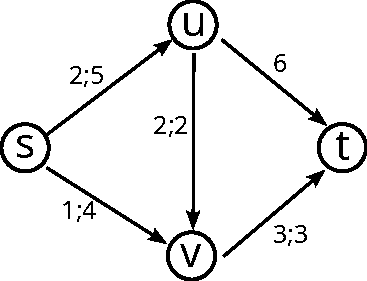
\includegraphics[height=40mm]{./images/flow9.pdf}\hfill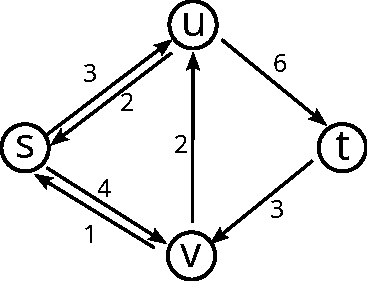
\includegraphics[height=40mm]{./images/flow10.pdf}
\begin{exampleblock}{Beispiel}
			\begin{itemize}
				\item links: der aktuelle Flu\ss\ im Ursprungsnetzwerk
				\item rechts: das Restnetzwerk
			\end{itemize}
		\end{exampleblock}
		\onslide<8>
		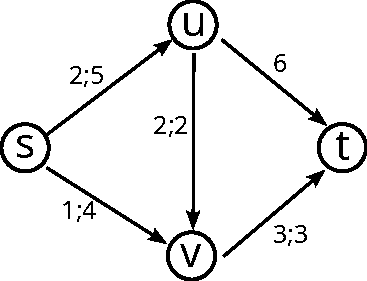
\includegraphics[height=40mm]{./images/flow9.pdf}\hfill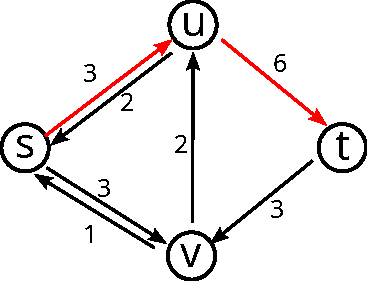
\includegraphics[height=40mm]{./images/flow11.pdf}
\begin{exampleblock}{Beispiel}
			\begin{itemize}
				\item links: der aktuelle Flu\ss\ im Ursprungsnetzwerk
				\item rechts: ein augmentierender Pfad mit Kapazit\"at drei
			\end{itemize}
		\end{exampleblock}
		\onslide<9>
		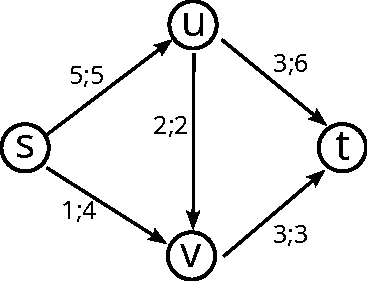
\includegraphics[height=40mm]{./images/flow12.pdf}\hfill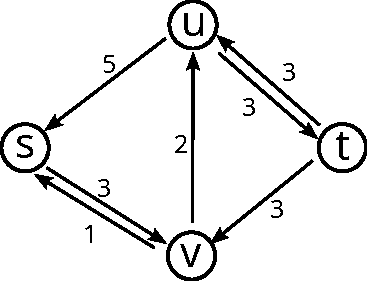
\includegraphics[height=40mm]{./images/flow13.pdf}
\begin{exampleblock}{Beispiel}
			\begin{itemize}
				\item links: der aktuelle Flu\ss\ im Ursprungsnetzwerk
				\item rechts: das Restnetzwerk
			\end{itemize}
		\end{exampleblock}
		\onslide<10>
		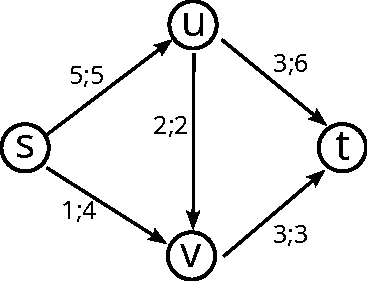
\includegraphics[height=40mm]{./images/flow12.pdf}\hfill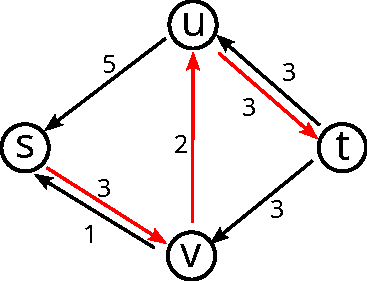
\includegraphics[height=40mm]{./images/flow14.pdf}
\begin{exampleblock}{Beispiel}
			\begin{itemize}
				\item links: der aktuelle Flu\ss\ im Ursprungsnetzwerk
				\item rechts: ein augmentierender Pfad mit Kapazit\"at zwei
			\end{itemize}
		\end{exampleblock}
		\onslide<11>
		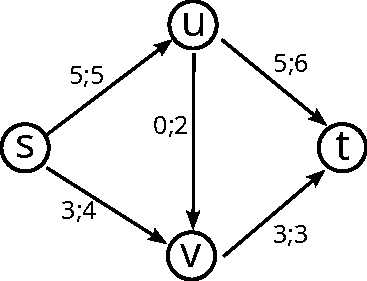
\includegraphics[height=40mm]{./images/flow15.pdf}\hfill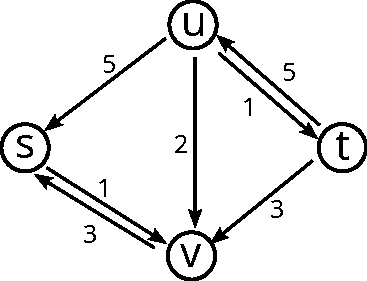
\includegraphics[height=40mm]{./images/flow16.pdf}
\begin{exampleblock}{Beispiel}
			\begin{itemize}
				\item links: der aktuelle Flu\ss\ im Ursprungsnetzwerk
				\item rechts: das Restnetzwerk; $t$ ist von $s$ nicht mehr erreichbar
			\end{itemize}
		\end{exampleblock}
	\end{overprint}
\end{frame}

\begin{frame}\frametitle{\mytitle}
	\begin{overprint}
		\onslide<1>
		\begin{exampleblock}{Schnitte}
			\begin{itemize}
				\item angenommen $N$ ist ein Netzwerk
				\item ein \alert{Schnitt} in $N$ ist eine Menge $S\subseteq V(G)$ mit
					$$s\in S\qquad\mbox{und}\qquad t\not\in S$$
				\item die \alert{Kapazit\"at} eines Schnittes $S$ ist
					\begin{align*}
						c(S)&=\sum_{(v,w)\in S\times (V\setminus S)}\vecone\{(v,w)\in E(G)\}c(v,w)
					\end{align*}
			\end{itemize}
		\end{exampleblock}
		\onslide<2>
		\hfill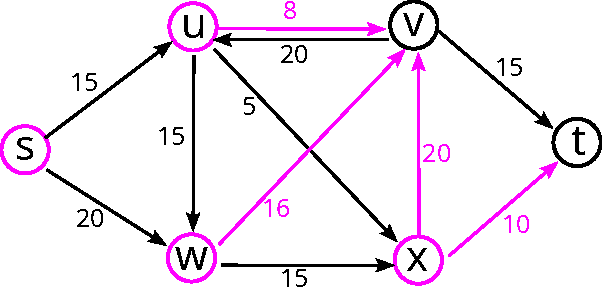
\includegraphics[height=40mm]{./images/flow17.pdf}
		\begin{exampleblock}{Beispiel}
			\begin{itemize}
				\item der Schnitt $S=\{s,u,w,x\}$ hat Kapazit\"at 54
			\end{itemize}
		\end{exampleblock}
		\onslide<3>
		\begin{block}{Lemma}
			Angenommen $N$ ist ein Netzwerk und $f$ ist ein Flu\ss\
			F\"ur jeden Schnitt $S$ gilt
			\begin{align*}
|f|=f(S,V\setminus S)
			\end{align*}
		\end{block}
		\begin{exampleblock}{Beweis}
			\vspace*{-4mm}
			\begin{align*}
				|f|&=f(s,V)\\
				   &=f(s,V)+f(S\setminus\{s\},V)&\mbox{[Flu\ss erhaltung]}\\
				   &=f(S,V)=f(S,V\setminus S)+f(S,S)\\
				   &=f(S,V\setminus S)&\mbox{[weil $f(S,S)=0$]}
			\end{align*}
		\end{exampleblock}
		\onslide<4>
		\begin{block}{Korollar}
			Wenn $N$ ein Netzwerk, $f$ ein Flu\ss\ und $S$ ein Schnitt ist, gilt $|f|\leq c(S)$
		\end{block}
		\begin{exampleblock}{Beweis}
			Das Lemma zeigt $|f|=f(S,V\setminus S)\leq c(S)$.
		\end{exampleblock}
	\end{overprint}
\end{frame}

\begin{frame}\frametitle{\mytitle}
	\begin{overprint}
		\onslide<1>
		\begin{block}{Theorem\hfill[``Max flow min cut theorem'']}
			F\"ur jedes Netzwerk $N$ gilt
			\begin{align*}
				\max\{|f|:f\mbox{ ist ein Flu\ss\ in $N$}\}&=\min\{c(S):S\mbox{ ist ein Schnitt in }N\}
			\end{align*}
		\end{block}
		\begin{exampleblock}{Beweis}
			\begin{itemize}
				\item wir suchen einen Flu\ss\ $f$ und einen Schnitt $S$ mit $|f|=c(S)$
				\item sei $f$ ist ein maximaler Flu\ss, d.h.\ $|f|=\max\{|\varphi|:\varphi\mbox{ ist ein Flu\ss\ in $N$}\}$
				\item angenommen es g\"abe einen augmentierenden Pfad $p$
				\item dann w\"are $|f+f_p|>|f|$; Widerspruch!
			\end{itemize}
		\end{exampleblock}
		\onslide<2>
		\begin{exampleblock}{Beweis}
			\begin{itemize}
				\item also gibt es keinen Pfad von $s$ nach $t$ in $N_f$
				\item betrachte daher die Menge
					\begin{align*}
						S&=\cbc{v\in V(G):\mbox{es gibt einen Pfad von $s$ nach $v$ in $N_f$}}
					\end{align*}
				\item dann ist $S$ ein Schnitt
				\item ferner gibt es keine Kante $(v,w)\in S\times (V\setminus S)$ in $N_f$
				\item folglich $f(v,w)=c(v,w)$ f\"ur alle $(v,w)\in S\times (V\setminus S)$ mit $(v,w)\in E(G)$
				\item also gilt $c(S)=|f|$
			\end{itemize}
		\end{exampleblock}
		\onslide<3>
		\begin{block}{Korollar}
			Wenn {\tt FordFulkerson} terminiert, ist die Ausgabe ein maximaler Flu\ss
		\end{block}
		\begin{exampleblock}{Beweis}
Wenn es keinen augmentierenden Pfad mehr gibt, ist $f$ ein maximaler Flu\ss
		\end{exampleblock}
		\begin{exampleblock}{Anmerkung}
			\begin{itemize}
				\item {\tt FordFulkerson} terminiert, wenn die Kapazit\"aten ganzzahlig sind
				\item allerdings kann dies $\max\{|f|:f\mbox{ Flu\ss\ in }N\}$ Schritte erfordern
				\item {\tt FordFulkerson} ist also nicht \emph{effizient!}
			\end{itemize}
		\end{exampleblock}
	\end{overprint}
\end{frame}

\begin{frame}\frametitle{\mytitle}
	\begin{overprint}
		\onslide<1>
		\begin{exampleblock}{Algorithmus {\tt EdmondsKarp}}
			\begin{itemize}
				\item verwende in {\tt FordFulkerson} Breitensuche, um den augmentierenden Pfad zu finden
				\item mit anderen Worte: finde jeweils einen \emph{k\"urzesten} augmentierenden Pfad
			\end{itemize}
		\end{exampleblock}
		\onslide<2>
		\begin{block}{Monotonielemma}
			Seien $f_1,f_2,\ldots$ die Fl\"usse, die {\tt EdmondsKarp} konstruiert.
			Sei ferner $\dist_{N_{f_i}}(s,v)$ der Abstand von $s,v$ im Restnetzwerk $N_{f_i}$.
			Dann gilt 
			\begin{align*}
				\dist_{N_{f_i}}(s,v)&\leq\dist_{N_{f_j}}(s,v)\qquad\mbox{f\"ur alle }i\leq j,\ v\in V(G).
			\end{align*}
		\end{block}
		\begin{exampleblock}{Beweis}
			\begin{itemize}
				\item angenommen nicht
				\item w\"ahle $i$ minimal mit $\dist_{N_{f_i}}(s,v)>\dist_{N_{f_{i+1}}}(s,v)$
				\item w\"ahle au\ss erdem $v$ so, da\ss\ $\dist_{N_{f_{i+1}}}(s,v)$ minimal ist
				\item sei ferner $p$ ein k\"urzester Pfad von $s$ nach $v$ in $N_{f_{i+1}}$
			\end{itemize}
		\end{exampleblock}
		\onslide<3>
		\begin{exampleblock}{Beweis}
			\begin{itemize}
				\item sei $u$ der letzte Knoten vor $v$ in $p$
				\item dann gilt $(u,v)\in N_{f_{i+1}}$ und $\dist_{N_{f_{i+1}}}(s,u)+1=\dist_{N_{f_{i+1}}}(s,v)$
				\item ferner gilt $\dist_{N_{f_{i+1}}}(s,u)\geq\dist_{N_{f_{i}}}(s,u)$ nach Wahl von $v$
				\item angenommen $(u,v)\in N_{f_i}$; dann gilt
					\begin{align*}
						\dist_{N_{f_{i}}}(s,v)&\leq\dist_{N_{f_{i}}}(s,u)+1\leq\dist_{N_{f_{i+1}}}(s,u)+1=\dist_{N_{f_{i+1}}}(s,v),
					\end{align*}
					im Widerspruch zur Wahl von $v$
			\end{itemize}
		\end{exampleblock}
		\onslide<4>
		\begin{exampleblock}{Beweis}
			\begin{itemize}
				\item weil $(u,v)\in N_{f_{i+1}}$ aber $(u,v)\not\in N_{f_i}$, mu\ss\ beim Augmentieren der Flu\ss\ von $v$ nach $u$ erh\"oht worden sein
				\item weil {\tt EdmondsKarp} entlang k\"urzester Pfade augmentiert, enth\"alt der k\"urzeste Pfad von $s$ nach $u$ in $N_{f_i}$ daher die Kante $(v,u)$
				\item daraus folgt aber
					\begin{align*}
						\dist_{N_{f_{i}}}(s,v)&=\dist_{N_{f_{i}}}(s,u)-1\leq\dist_{N_{f_{i+1}}}(s,u)-1=\dist_{N_{f_{i+1}}}(s,v)-2,
					\end{align*}
					im Widerspruch zur Wahl von $v$
			\end{itemize}
		\end{exampleblock}
		\onslide<5>
		\begin{block}{Satz}
			{\tt EdmondsKarp} hat Laufzeit $O(|V(G)|\cdot|E(G)|^2)$
		\end{block}
		\begin{exampleblock}{Beweis}
			\begin{itemize}
				\item wir zeigen, da\ss\ {\tt EdmondsKarp} nach h\"ochstens $O(|V(G)|\cdot|E(G)|)$ Augmentierungen terminiert
				\item weil Breitensuche jeweils Zeit $O(|E(G)|)$ ben\"otigt, folgt daraus der Satz
				\item eine Kante $(v,w)$ auf einem augmentierenden Pfad $p$ ist \alert{kritisch} f\"ur einen Flu\ss\ $f$, falls $c_f(v,w)=c_f(p)$
				\item dann ist $(v,w)$ nicht in $N_{f+f_p}$ enthalten
				\item wir zeigen, da\ss\ keine Kante mehr als $|V(G)|/2$ mal kritisch werden kann
			\end{itemize}
		\end{exampleblock}
		\onslide<6>
		\begin{exampleblock}{Beweis}
			\begin{itemize}
				\item angenommen $(v,w)$ wird kritisch f\"ur eine Flu\ss\ $f$ f\"ur den Pfad $p$, den {\tt EdmondsKarp} ausw\"ahlt
				\item weil $p$ ein k\"urzester Pfad ist, gilt f\"ur die Abst\"ande in dem Netzwerk $N_f$:
					\begin{align*}
						\dist_{N_f}(s,w)>\dist_{N_f}(s,v)
					\end{align*}
				\item angenommen $(v,w)$ wird sp\"ater noch einmal kritisch
				\item dann mu\ss\ die Kante $(v,w)$ zun\"achst wieder in das Restnetzwerk eingef\"ugt worden sein
				\item dies ist nur m\"oglich, wenn die Kante $(w,v)$ auf dem augmentierenden Pfad f\"ur einen Flu\ss\ $f'$ gelegen hat
				\item f\"ur den Flu\ss\ $f'$ gilt dann $\dist_{N_{f'}}(s,v)>\dist_{N_{f'}}(s,w)$
				\item das Monotonielemma zeigt also
					\begin{align*}
						\dist_{N_{f'}}(s,v)\geq\dist_{N_f}(s,v)+2
					\end{align*}
			\end{itemize}
		\end{exampleblock}
		\onslide<7>
		\begin{exampleblock}{Beweis}
			\begin{itemize}
				\item das Monotonielemma zeigt also
					\begin{align*}
						\dist_{N_{f'}}(s,v)\geq\dist_{N_f}(s,v)+2
					\end{align*}
				\item weil $\dist_{N_{f'}}(s,v)\leq|V(G)|$, kann $(v,w)$ also nur $|V(G)|/2$ mal kritisch werden
			\end{itemize}
		\end{exampleblock}
	\end{overprint}
\end{frame}

\begin{frame}\frametitle{\mytitle}
	\begin{overprint}
		\onslide<1>
		\begin{exampleblock}{Matchings}
			\begin{itemize}
				\item ein \alert{Matching} in einem ungerichteten Graphen $G=(V,E)$ ist eine Menge $M\subseteq E$ von Kanten, so da\ss
					\begin{align*}
						e\cap f&=\emptyset\qquad\mbox{f\"ur alle }e,f\in M,\,e\neq f
					\end{align*}
				\item mit $\nu(G)$ wird die maximale Gr\"o\ss e eines Matchings in $G$ bezeichnet (``Matchingzahl von $G$'')
				\item $G$ hei\ss t \alert{bipartit}, falls $\chi(G)=2$
				\item eine \alert{Bipartition} von $G$ ist ein Paar $(S,T)$ von stabilen Mengen, so da\ss\ $S\cup T=V(G)$ und $S\cap T=\emptyset$
			\end{itemize}
		\end{exampleblock}
		\onslide<2>
		\begin{exampleblock}{Satz von Hall}
			Sei $G$ ein bipartiter Graph mit Bipartition $(S,T)$.
			Es gilt $\nu(G)=|S|$ genau dann, wenn
			\begin{align*}
				|\partial U|\geq|U|\qquad\mbox{f\"ur alle }U\subseteq S.
			\end{align*}
			\emph{Erinnerung:} $\partial U=\{v\in V(G):\exists u\in U:v\in\partial u\}$
		\end{exampleblock}
		\onslide<3>
		\begin{exampleblock}{Beweis}
			\begin{itemize}
				\item wenn $\nu(G)=|S|$, dann gilt $|\partial U|\geq|U|$ f\"ur alle $U\subseteq S$
				\item nehme nun umgekehrt an, da\ss\ $|\partial U|\geq|U|$ f\"ur alle $U\subseteq S$
				\item konstruiere ein Netzwerk $N=(\Gamma,c,s,t)$, so da\ss\
					\begin{align*}
						V(\Gamma)&=V(G)\cup\{s,t\}\qquad\mbox{mit}\qquad s,t\not\in V(G)\\
						E(\Gamma)&=\{(v,w)\in S\times T:vw\in E(G)\}\cup\{s\}\times S\cup T\times\{t\}
					\end{align*}
				\item ferner ist $c(v,w)=1$ f\"ur alle $(v,w)\in E(\Gamma)$
			\end{itemize}
		\end{exampleblock}
		\onslide<4>
		\begin{exampleblock}{Beweis}
			\begin{itemize}
				\item sei nun $f:V(\Gamma)\times V(\Gamma)\to\{0,1\}$ ein maximaler Flu\ss
				\item dann ist
					\begin{align*}
						M&=\{vw\in E(G):f(v,w)=1\}
					\end{align*}
					ein Matching von $G$
				\item zu zeigen ist also, da\ss\ $|f|=|S|$
				\item nach dem max flow min cut theorem gen\"ugt es zu zeigen, da\ss\ f\"ur jeden Schnitt $Y$ von $N$ gilt
					$$c(Y)\geq|S|$$
			\end{itemize}
		\end{exampleblock}
		\onslide<5>
		\begin{exampleblock}{Beweis}
			\begin{itemize}
				\item definiere daher $A=Y\cap S$ und $B=Y\cap T$
				\item nach Konstruktion von $N$ gilt dann
					\begin{align*}
						c(Y)\geq|S\setminus A|+|\partial A|
					\end{align*}
				\item weil ferner $|\partial A|\geq|A|$, folgt $c(Y)\geq|S|$
			\end{itemize}
		\end{exampleblock}
		\onslide<6>
		\begin{exampleblock}{Matchings via Fl\"usse}
			\begin{itemize}
				\item mit der Konstruktion eines Netzwerkes aus dem Beweis erhalten wir ein effizientes Verfahren, um die Matchingzahl bipartiter Graphen zu berechnen
				\item wir wenden auf dieses Netzwerk einfach {\tt FordFulkerson} an
				\item da alle Kapazit\"aten $\{0,1\}$ sind, ist der optimale Flu\ss\ auch $\{0,1\}$-wertig
				\item \itshape es gibt effizientere Algorithmen f\"ur dieses Problem $\leadsto$ VL Effiziente Algorithmen
			\end{itemize}
		\end{exampleblock}
	\end{overprint}
\end{frame}

\begin{frame}\frametitle{\mytitle}
	\begin{overprint}
		\onslide<1>
		\begin{exampleblock}{Zusammenfassung}
			\begin{itemize}
				\item Fl\"usse in Netzwerken
				\item {\tt FordFulkerson} und {\tt EdmondsKarp}-Algorithmen
				\item max flow min cut
				\item Matchings in bipartiten Graphen
			\end{itemize}
		\end{exampleblock}
	\end{overprint}
\end{frame}

\end{document}
